\chapter{Struktura Aplikacji}

Struktura aplikacji została częściowo opisana w rozdziale \hyperref[ch:manual]{\textbf{Podręcznik użytkownika}}.

\section{Edytor notatki}

Edytor notatki składa się z edytora tytułu znajdującego się w głównym pasku strony edycji notatki, oraz edytora zawartości.

\subsection{Zarządzanie zawartością}

Do zarządzania zawartością notatki używana jest klasa \textbf{NoteParagraphs} przechowująca listę obiektów typu \textbf{NoteParagraph} reprezentujących paragrafy notatki.
Współpracę tych klas można przedstawić w uproszczony sposób za pomocą schematu:

\begin{figure}[ht]
    \centering
    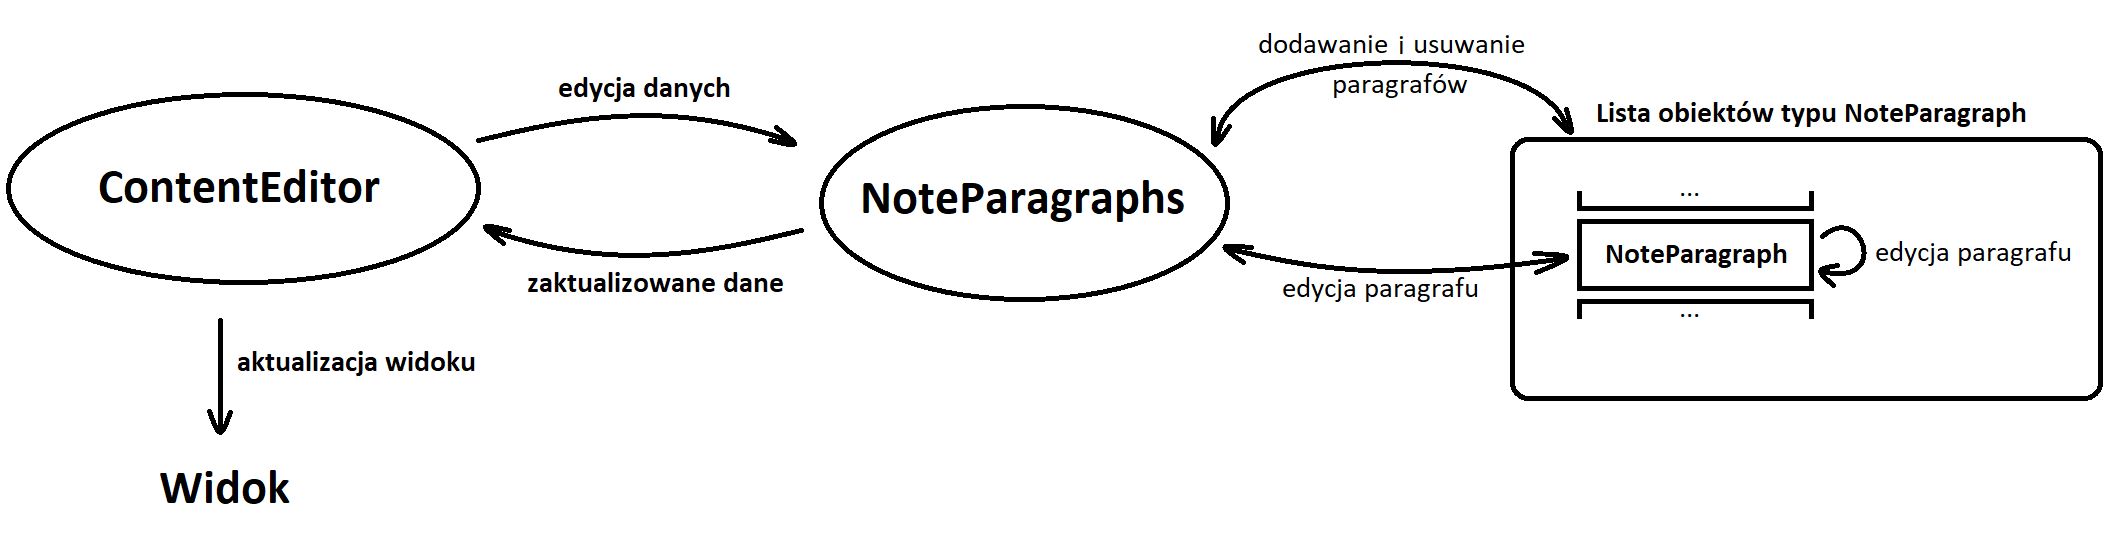
\includegraphics[width=\linewidth]{images/ContentEditor_podzial.png}
    \caption{Uproszczony schemat zarządzania paragrafami.}
\end{figure}

\newpage

\subsection{Paragrafy}

Istanieją trzy typy paragrafów w edytorze dziedziczące po \textbf{NoteParagraph}: 
\begin{itemize}
    \item \textbf{NoteParagraphTextEditor},
    \item \textbf{NoteParagraphWidget},
    \item \textbf{NoteParagraphPlaceholder}
\end{itemize}

Każdy z paragrafów posiada unikalny identyfikator \textbf{id} oraz referencję do fabryki widgetów tworzonej wewnątrz managera \textbf{NoteParagraphs}.
Pozwala to na unikalne identyfikowanie paragrafów wewnątrz listy, oraz wszystkich utworzonych widgetów w obrębie przestrzenii edytora.

Używane są również mechanizmy wywołań zwrotnych(callbacks) do zgłaszania aktywności(focus), zaistniałej zmiany, jak również usunięcia samego siebie z listy paragrafów, na podstawie swojego id, gdy wszystkie jego elementy zostaną usunięte.

\subsubsection{NoteParagraphTextEditor}

Służy do przechowywania, wyświetlania i edycji tekstu notatki. Posiada mechanizmy dynamicznej zmiany rozmiaru poprzez manipulację stanem oraz wartościami wewnętrznych pól. Posiada tylko jeden element, którym jest pole tekstowe z niestandardowym kontrolerem parsującym tekst przy użyciu własnego parsera.

\subsubsection{NoteParagraphWidget}

Służy do przechowywania, wyświetlania i edycji widgetów notatki. Posiada mechanizmy dynamicznej zmiany rozmiaru wraz ze zmianą rozmiaru widgetu będącego elementem głównym. Mechanizmy zmiany rozmiaru są różne w zależności od rodzaju widgetu.

\subsubsection{NoteParagraphPlaceholder}

Służy jako wypełnienie pozostałej przestrzeni edytora. Po kliknięciu na niego uruchamia mechanizm przenoszenia aktywności(focus) na ostatni paragraf na liście, dzięki czemu użytkownik nie musi znać wielkości i szukać ostatniego paragrafu, aby kontynuować edycję notatki.

\section{Praca z tekstem}

Praca z tekstem dzieli się na edycję tekstu z użyciem logiki zawartej w \textbf{NoteParagraphTextEditor} i \textbf{NoteTextEditorWidget}, jak również wyświetlanie go wraz ze zmianą rozmiarów z pomocą \textbf{NoteTextEditingController}.

\subsection{Edycja Tekstu}

Tekst edytowany jest za pomocą pola tekstowego TextField udostępnianego jako widget przez framework flutter. Posiada on wewnętrzny padding poziomy(lewa i prawa strona) jako stałą wartość, oraz padding pionowy(góra, dół) obliczany na podstawie różnicy pomiędzy wielkoścą czcionki użytej w danym paragrafie, a domyślnej czcionki z dodatkiem podstawowej wartości niezerowej(w przypadku, gdy dany paragraf nie ma ustawionego nagłówka, nie chcemy braku odstępu między paragrafami z powodu zerowego paddingu pionowego).

Przy każdej zmianie tekstu sprawdzana jest jego zawartość w poszukiwaniu informacji o stanie paragrafu. Stan ten określa się poprzez wielkośc czcionki i stylów tekstu użytych w paragrafie.

\subsubsection{Dodawanie tekstu}

Jeśli wewnątrz pola tekstowego został dodany znak nowej linii, wówczas wołane jest wywołanie zwrotne(callback), zainicjalizowane przy tworzeniu danego paragrafu przez \textbf{NoteParagraphs}, do dodawania nowego paragrafu. Wywołanie to przyjmuje identyfikator danego paragrafu i na tej podstawie oblicza miejsce w liście do którego należy włożyć nowopowstały paragraf. Przy tworzeniu nowego paragrafu następuje przeniesienie tekstu następującego po znaku końca linii. Znak końca linii jest usuwany.

\subsubsection{Usuwanie tekstu}
\label{eq:usuwanieTekstu}

Flutter nie oferuje możliwości przechwycenia zdarzenia naciśnięcia przycisku \textbf{delete}, gdy kursor znajduje się na początku tekstu. W tej sytuacji najprościej jest użyć przechwycenia zdarzenia edycji tekstu w paragrafie.

W każdym paragrafie na początku dodawany jest znak \verb|placeholder = \u200b|. Jest to znak unicode reprezentujący spację o zerowej długości, a więc niewidoczną w tekście. Jest to swego rodzaju wartownik, którego brak na początku tekstu podczas sprawdzania tekstu po edycji, mówi o potrzebie usunięcia paragrafu.

Gdy użytkownik zechce usunąć paragraf, wówczas przenosi się kliknięciem na początek wiersza(o ile już się na nim nie znajduje), a następnie naciska przycisk \textbf{delete}. Dzięki temu usuwa \verb|placeholder|, a przy tym wywoływany jest callback służący do usunięcia paragrafu. Jako argument przyjmuje identyfikator paragrafu, aby określić miejsce usunięcia.

Aby uniknąć kliknięcia na początek linii, przed wartownika, dodany został mechanizm zmiany pozycji kursora na drugi znak(bezpośrednio za wartownikiem) za każdym razem gdy jest on na pozycji zerowej.

\subsection{Wyświetlanie tesktu}

Do wyświetlania stylizowanego tekstu używane są obiekty typu \textbf{TextSpan}. Obiekty te posiadają drzewiastą strukturę, ponieważ mogą zawierać dzieci tego samego typu, które będą dziedziczyć dane parametry stylu, o ile nie zostaną dla nich specjalnie zainicjalizowane. Daje to możliwość zorganizowania tesktu bez potrzeby dzielenia go na małe kawałki oraz nadawania za każdym razem łączonych styli(gdyby obiekty \textbf{TextSpan} były przechowywane jako elementy jednej listy). Można zainicjalizować jeden styl wewnątrz drugiego, co bardzo upraszcza strukturę i pozwala na wprowadzanie globalnych zmian struktury(jak na przykład wielkość czcionki całego paragrafu) tylko w korzeniu, zapewniając, że wszystkie części tekstu odziedziczą zmianę.

Aktualizacja i renderowanie wyglądu pola tekstowego na bieżąco jest możliwe poprzez wykorzystanie klasy \textbf{TextEditingController}. Posiada ona metodę \textbf{buildTextSpan}, która służy do budowania wyglądu i stylu tekstu poprzez obiekty \textbf{TextSpan}. Dzieczicząc z tej klasy i nadpisując metodę \textbf{buildTextSpan} mogłem użyć parsera tekstu zawierającego znaczniki do przekonwertowania go na stylizowany tekst.
Dzięki temu przy każdej zmianie tekst jest parsowany, a jego wygląd aktualizowany.

Utworzony w ten sposób \textbf{NoteTextEditingController} może nie tylko używać parsera do tworzenia obiektów \textbf{TextSpan}, ale również mógł zostać rozszerzony o dodatkowe parametry, takie jak:

\begin{compactitem}
    \item callback \textbf{resizeTextField} wołany podczas parsowania, gdy wielkość czcionki w tekście ulega zmianie, 
    \item możliwość przechowywania informacji o tym, czy dany paragraf jest aktualnie w użyciu,
    \item sprawdzanie i manipulacja pozycją kursora.
\end{compactitem}

Callback \textbf{resizeTextField} został użyty w kontrolerze, zamiast w widgecie pola tekstowego, ponieważ wtedy wystarczy parsować tekst jednokrotnie. Przed samym zwróceniem drzewiastej struktury tekstu \textbf{TextSpan} możemy ustawić rozmiar pola tekstowego w jego korzeniu, zamiast edytować zawartość widgetu w innych mechanizmach i tak czy inaczej parsować dodatkowo tekst w poszukiwaniu informacji na temat wielkości czcionki.

Informacja na temat aktualnego użycia paragrafu jest używana do wyświetlania i ukrywania znaczników stylu nagłówka.

Sprawdzanie i manipulacja pozycją kursora pozwala na odkrywanie znaczników stylu, jak również ustawianie pozycji, aby kursor nie znajdował się przed znakiem \verb|placeholder|(zobacz \hyperref[eq:usuwanieTekstu]{Usuwanie tekstu}).

Przy każdej zmianie tekstu odświeżany jest widok paragrafu, dlatego wystarczy zmienić wartość zmiennej odpowiadającej za jego rozmiar przed końcem całej operacji związanej z przetwarzaniem nowego tekstu.
%https://api.flutter.dev/flutter/widgets/TextEditingController/buildTextSpan.html

\subsection{Problem parsowania tekstu ze znacznikami stylu}

Do wyświetlania stylizowanego tekstu potrzebne jest jego parswoanie. Funkcjonalnośc ta, będzie wołana stosunkowo często, a dla długich tekstów bez znaku nowej linii będzie to długi do obsługi tekst. Dlatego też ważny jest sposób implementacji.

Zrealizowanym pomysłem rozwiązania problemu jest podział parsowania tekstu na trzy etapy:
\begin{enumerate}
    \setlength\itemsep{0mm}
    \item przkształcanie znaczników stylu w tekście na \textbf{znaki unicode}
    \item parsowanie tekstu ze \textbf{znakami unicode} na specjalną drzewiastą reprezentację \textbf{SpanInfo}
    \item konwersja struktury \textbf{SpanInfo} na obiekt \textbf{TextSpan}
\end{enumerate}

\subsection{Implementacja Parsera}

\subsubsection{Własna implementacja}

Parser wraz z jego strukturą został zaprojektowany i zaimplementowany przeze mnie, zamiast przy użyciu narzędzi generowania parsera dla opisanej gramatyki użwanego przeze mnie języka znaczników. Powodem tego jest potrzeba łatwego rozwoju oraz wprowadzenia niestandardowych rozwiązań i dodatkowych funkcjonalności niebędących częścią samej składni gramatyki, jednak potrzebnych wewnątrz implementacji parsera.

Własna implementacja parsera pozwoliła mi od początku do końca zaprojektować i zrozumieć jego strukturę co pozwoliło mi tworzyć elastyczne środowisko rozwoju tekstu w notatkach. Przykładowo wprowadzanie funkcji odkrywania i ukrywania znaczników stylu oraz nagłówka, bądź dodanie wywołania zwrotnego zmieniającego rozmiar pola tekstowego, było prostym zabiegiem niewymagającym dużych zmian i rozrzerzeń kodu parsera.

\subsubsection{Parsowanie}

Każdy z etapów parsowania jest realizowany poprzez inną klasę. Całość łączona jest w metodzie obiektu \textbf{NoteTextEditingController}.
\newline
\begin{figure}[ht]
    \centering
    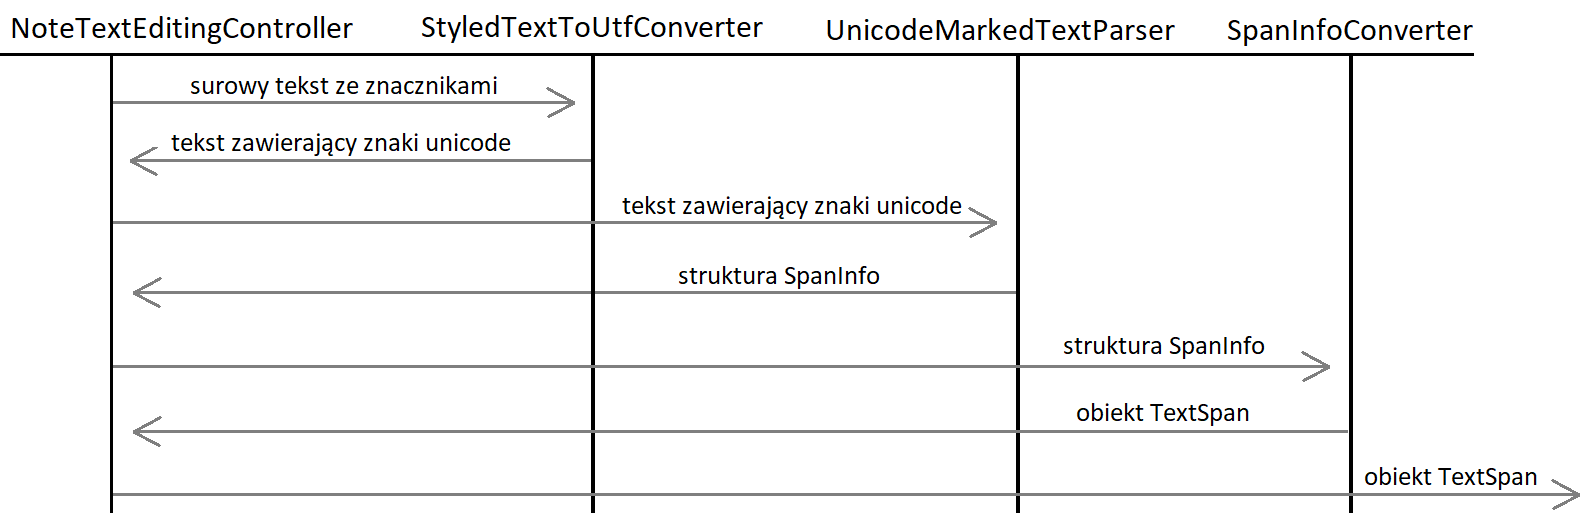
\includegraphics[width=\linewidth]{images/etapy_parsowania.png}
    \caption{Schemat przedstawiający etapy parsowania tekstu.}
    \label{fig:etapyParsowania}
\end{figure}

\subsubsection{Znaki unicode}

%https://unicode.org/glossary/#private_use_area
Do procesu parsowania zostały użyte znaki unicode z bloku Private Use Area(Prywatny Obszar Użytkowania). Są to znaki, które są trudno dostępne dla użytkownika z poziomu klawiatury mobilnej.

\noindent Zdefiniowane zostały w następujący sposób:

\begin{lstlisting}[language=java]
const styleUnicodeNumber = 0xe000;
const widgetUnicodeNumber = 0xe100;
const elementUnicodeNumber = 0xe1A0;
const paragraphUnicodeNumber = 0xe200;
\end{lstlisting}

Oznaczają odpowiednio początki przestrzeni znaczników: stylu tekstu, wewnętrznych widgetów i elementów w tekście oraz nagłówków paragrafu.
Znaczniki początkowe mają parzyste numery, natomiast znaczniki końcowe mają nieparzyste numery następujące po odpowiadających im znacznikach początkowych.

\newpage

\subsubsection{Struktura SpanInfo}

Podczas implementacji użyta została struktura \textbf{SpanInfo}. Zawiera ona informacje na temat danego węzła w drzewiastej strukturze stylów tekstu, oraz referencję do jego rodzica.
Została zaimplementowana w celu usprawnienia przebiegu etapu drugiego parsowania tekstu.

\begin{lstlisting}[language=java]
class SpanInfo {
  String type;
  String text;
  List<SpanInfo> children;
  late SpanInfo parent;
}
\end{lstlisting}

Dzięki swojej budowie struktura może zostać przekonwertowana w prosty sposób na obiekt typu \textbf{TextSpan}.

\subsubsection{StyledTextToUtfConverter}

Przekształcanie znaczników odbywa się poprzez przejście przez tekst w ich poszukiwaniu i przetwarzaniu. Znaczniki dzielone są na początkowe i końcowe(zobacz: \hyperref[subsec:ustawianieStyli]{Ustawianie styli}). Podczas sprawdzania czy dany znak jest znacznikiem początkowym, czy końcowym pobierany jest szerszy kontekst, złożony z przylegających do niego znaków.

W momencie, gdy zostanie znaleziony znak będący początkowym znacznikiem, dodawana jest informacja o nim do listy \textbf{startBounds} w postaci struktury \textbf{SpecialPatternInfo} przechowującej znacznik wraz z jego indeksem.

\begin{lstlisting}[language=Java]
class SpecialPatternInfo {
  final int indexInText;
  final String character;
}
\end{lstlisting}

W przypadku znalezienia znaku $c$ będącego końcowym znacznikiem, przeszukujemy listę \textbf{startBounds} w poszukiwaniu pierwszego wystąpienia znacznika $c'$ o takiej samej wartości. Jeśli nie zostanie znaleziony, wówczas znak $c$ traktowany jest jako zwykły tekst. Jesli natomiast zostanie znaleziony, oznacza to, że wystąpił wcześniej początek stylu, a cały tekst pomiędzy aktualnym indeksem, a indeksem zapisanym w strukturze opisującej początkowy znacznik $c'$ jest tekstem zawierającym ten styl. Zatem znalezione znaczniki zamieniane są na swoje odpowiedniki w formie znaków unicode, a znaczniki istniejące na liście będące następnikami znalezionego $c'$ zostają usunięte z listy(style nie mogą się przecinać), a więc nie zostaną zamienione.

W podobny sposób konwertowane są również widgety i elementy wewnętrzne w tekście. W aktualnej wersji aplikacji nie są one obsługiwane, jednak sam parser został przygotowany na obsługę tego typu problemu. Szukane są zatem również fragmenty tekstu będące tagami widgetów bądź oznaczeniami elementów.

\subsubsection{UnicodeMarkedTextParser}

Z racji tego, ze znaki unicode z tego zakresu są trudno dostępne, na potrzeby samego problemu konwersji tekstu notatek możemy założyć, że znaki w tekście symbolizują początkowe i końcowe znaczniki, które na pewno mają swoje odpowiedniki i są poprawnie użyte(nie przecinają się).

Na początku algorytmu tworzona jest referencja $currentSpan$ na obiekt \textbf{SpanInfo}, który jest aktualnie przetwarzanym stylem(napotkany został jego znacznik początkowy). Początkowo jest to korzeń całej struktury \textbf{SpanInfo}.

Oznaczony w ten sposób tekst przechodzimy ponownie, jednak posiadając dokładne informacje, które symbole są znacznikami stylu, a które zwykłymi fragmentami tekstu.

Podczas przechodzenia tekstu zapisujemy znaki niebędące znacznikami do tymczasowego bufora.

Napotykając znacznik początkowy, jeśli w buforze znajduje się tekst, to wówczas jest on dodawany do tekstu przechowywanego w $currentSpan$. Następnie tworzony jest nowy \textbf{SpanInfo}, na podstawie stylu reprezentowanego przez znacznik, będący dzieckiem $surrentSpan$ i zapisywany jest jako $currentSpan$. 

Po napotkaniu znacznika końcowego dodajemy tekst z tymczasowego bufora do $currentSpan$, czyścimy bufor i przestawiamy $currentSpan$ przechodząc po węzłach \textbf{SpanInfo}(używane jest do tego pole z referencją $parent$ wskazującą na rodzica danego węzła) na pierwszy napotkany węzeł przechowujący informacje na temat stylu reprezentowanego przez aktualnie sprawdzany znacznik.

Przetwarzane są również informacje na temat widgetów i elementów wewnętrznych przygotowane w ramach podstawy do rozwoju funkcjonalności w przyszłosci.

\subsubsection{SpanInfoConverter}

Klasa \textbf{TextSpan} jest klasą pochodną klasy \textbf{InlineSpan}.

\textbf{SpanInfoConverter} buduje strukturę \textbf{InlineSpan} złożoną z obiektów klas pochodnych \textbf{TextSpan} oraz \textbf{WidgetSpan}. Biorąc pod uwagę, że wewnętrzne widgety i elementy, które mają w przyszłości być obsługiwane przy użyciu \textbf{WidgetSpan} nie są aktualnie obsługiwane przyjęty w opisie model struktury opiera się tylko na obiektach typu \textbf{TextSpan}.

Przechodząc przez strukturę \textbf{SpanInfo} budujemy strukturę złożoną z obiektów typu \textbf{TextSpan}. Zapisywany jest $mainSpan$ będący korzeniem struktury, natomiast przejście przez strukturę odbywa się w sposób rekurencyjny.

\begin{lstlisting}[language=Java]
SpanInfo mainSpan = SpanInfo(type: 'null');

InlineSpan getSpans(SpanInfo spanInfo) {
    if (mainSpan.type == 'null') mainSpan = spanInfo;

    List<InlineSpan> spanChildren =
        spanInfo.children.map((e) => getSpans(e)).toList();

    /* ustawianie stylu i typu obiektu 
     * oraz zwracanie go wraz z children */
}
\end{lstlisting}

\section{Praca z widgetami}



